\documentclass{article}
\usepackage[utf8]{inputenc}
\usepackage{amsmath}
\usepackage{braket}
\usepackage{gensymb}
\usepackage{amssymb}
\usepackage{natbib}
\usepackage{graphicx}
\usepackage{listings}
\usepackage{color}
\usepackage{tikz}
\usepackage{multicol}
\usetikzlibrary{arrows}
\usepackage{float}
\restylefloat{figure}

\usepackage[figurename=Figure]{caption}

\definecolor{codegreen}{rgb}{0,0.6,0}
\definecolor{codegray}{rgb}{0.5,0.5,0.5}
\definecolor{codepurple}{rgb}{0.58,0,0.82}
\definecolor{backcolour}{rgb}{0.95,0.95,0.92}
 
\lstdefinestyle{mystyle}{
    backgroundcolor=\color{backcolour},   
    commentstyle=\color{codegreen},
    keywordstyle=\color{magenta},
    numberstyle=\tiny\color{codegray},
    stringstyle=\color{codepurple},
    basicstyle=\footnotesize,
    breakatwhitespace=false,         
    breaklines=true,                 
    captionpos=b,                    
    keepspaces=true,                 
    numbers=left,                    
    numbersep=5pt,                  
    showspaces=false,                
    showstringspaces=false,
    showtabs=false,                  
    tabsize=2
}
 
\lstset{style=mystyle}
\lstset{
    language=Erlang,
    mathescape=true
}
\usepackage{hyperref}
\hypersetup{
    colorlinks=true,
    linkcolor=blue,
    filecolor=magenta,      
    urlcolor=cyan,
}

\title{FYS2130 - Project}
\author{Candidate - 15266}
\date{April 2018}

\begin{document}

\maketitle

\section*{Problems}

\subsection*{Problem 1}
We are asked to solve the equation
\begin{equation}
ma(t) + kx(t) = 0,
\end{equation}
numerically using the Runge-Kutta 4 method where we have written the code ourself. We start by setting up an expression we can feed into our function, which is basicly just to solve for $a$
\begin{equation}
a(t) = -\frac{k}{m}x(t).
\end{equation}
Using the constants and initial conditions given in the problem
\begin{figure}[H]
\centering
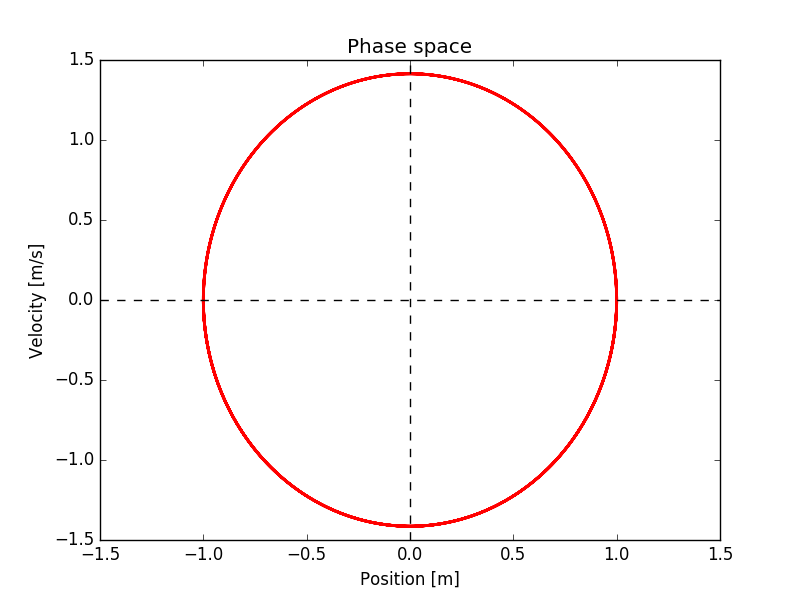
\includegraphics[width=0.6\textwidth]{problem_1_1}
\caption{Phase diagram of a harmonic oscilator.}
\label{fig:problem_b_contour_fig}
\end{figure}


\subsection*{Problem 2}



\subsection*{Problem 3}
\begin{equation}
mx'' + kx
\end{equation}

\subsection*{Problem 4}

\subsection*{Problem 5}

\subsection*{Problem 6}

\subsection*{Problem 7}

\subsection*{Problem 8}

\subsection*{Problem 9}

\section*{Appendix}

\subsection*{Python code}
\hypertarget{pythonsourcecode}{}
\lstinputlisting[language=Python]{code.py}


\end{document}

